\documentclass{article}

%Packages
\usepackage{graphicx}
\usepackage{url}

%Standart stuff
\title{Status Quo der digitalen Gesundheitsanwendungen}
\author{Marcelo Hauger}
\date{\today}

\begin{document}
	\maketitle
	\newpage
	\tableofcontents
	\newpage
	\section{Grundlagen}
		Durch das Inkrafttreten des Digitale-Versorgung-Gesetzes (DVG) am 19. Dezember 2019 wurden Digitale Gesundheitsanwendungen für Patienten in die Gesundheitsversorgung eingeführt (§§ 33a und 139e Fünftes Buch Sozialgesetzbuch). Ungefähr 73 Millionen Versicherte in der gesetzlichen Krankenversicherung haben Anspruch auf DiGA-Versorgung, die von Ärzten und Psychotherapeuten verordnet und von der Krankenkasse erstattet werden können.
		\subsection{Was ist eine "DiGA"?}
			DiGA (Digitale Gesundheitsanwendung), als "digitale Helfer" in der Hand der Patientinnen und Patienten, bieten zahlreiche Möglichkeiten, Krankheiten zu erkennen und zu behandeln sowie den Weg zu einer selbstbestimmten, gesundheitsförderlichen Lebensführung zu unterstützen. Die DiGA müssen als CE-gekennzeichnetes Medizinprodukt folgende Eigenschaften mit sich bringen:
			\begin{itemize}
				\item Ein Medizinprodukt der Risikoklasse 1 oder 2a nach MDR (Medical Device Regulation) und im Rahmen der Übergangsvorschriften nach MDD (Medical Device Directive).
				\item Die Hauptfunktion basiert auf digitalen Technologien.
				\item Der medizinische Zweck wird wesentlich durch die digitale Hauptfunktion erreicht.
				\item Die DiGA unterstützt die Erkennung, Überwachung, Behandlung oder Linderung von Krankheiten oder die Erkennung, Behandlung, Linderung oder Kompensierung von Verletzungen oder Behinderungen.
				\item Die DiGA wird entweder vom Patienten, oder vom Leistungserbringer und Patient gemeinsam genutzt.
			\end{itemize}  
			Diese Anforderungen sind in § 33a Fünftes Buch Sozialgesetzbuch (SGB V) definiert.\cite[vgl. Was ist eine DiGA?]{wissenswertes-diga}. Sollten alle Anforderungen erfüllt sein, wird entsprechende DiGA in das sogenannte "DiGA-Verzeichnis" aufgenommen. Dort sind alle DiGAs gelistet die obengenannte Anforderungen erfüllt haben.   
		\newpage
		\subsection{Fast-Track-Verfahren} 
			\begin{figure}[htbp]
				\centering
				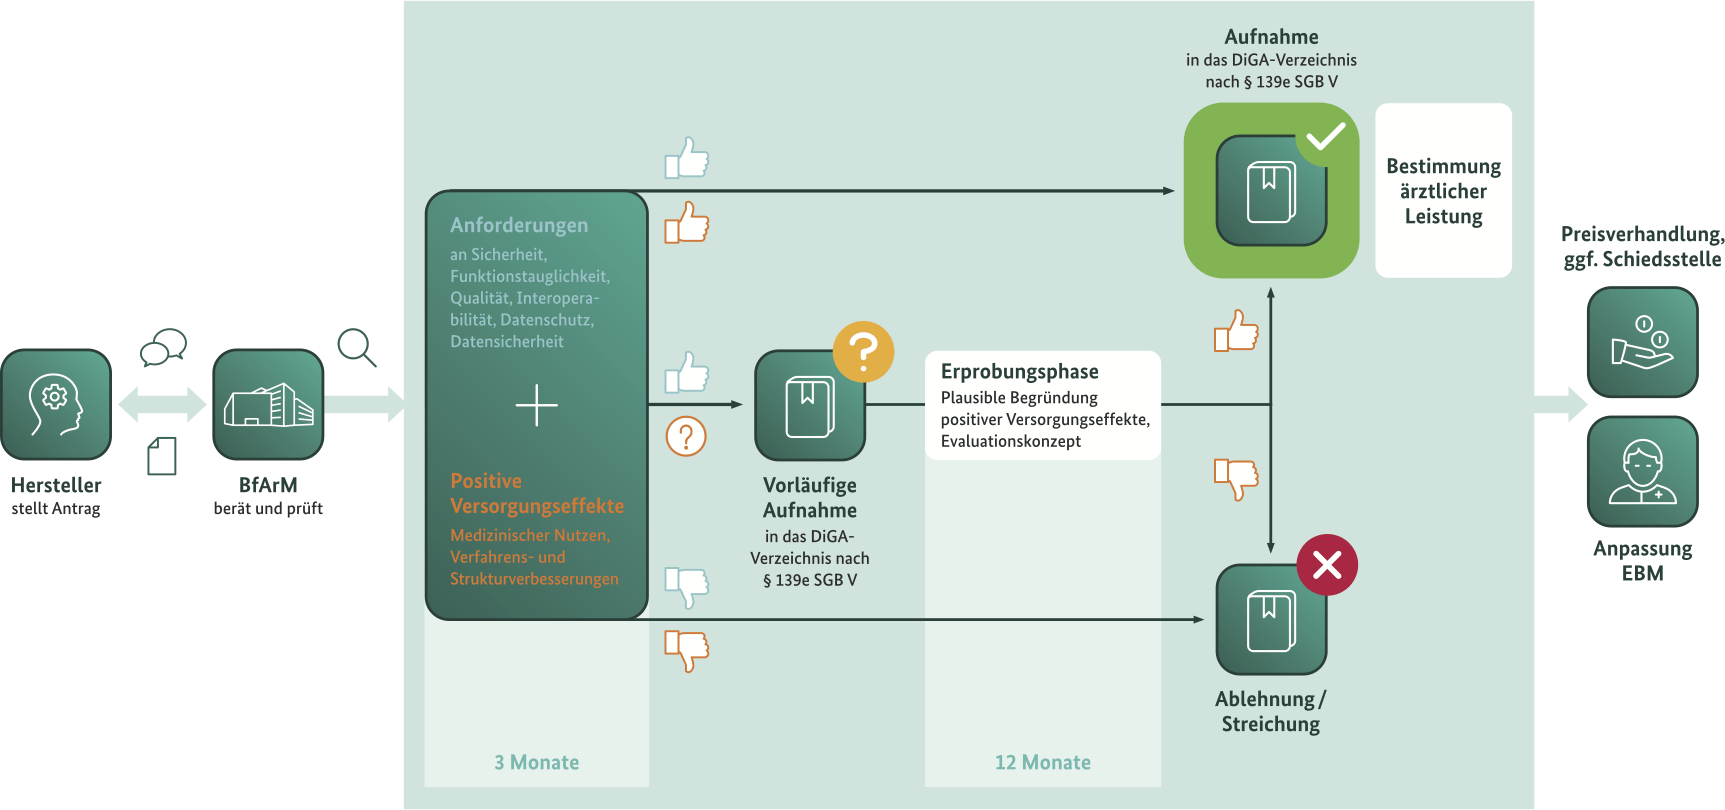
\includegraphics[width=0.75\textwidth]{./grafiken/fast-track-verfahren}
				\caption[Ablaufdiagramm des Fast-Track-Verfahren]{Ablaufdiagramm des Fast-Track-Verfahren}
				\label{Abb-ft-Verfahren}
			\end{figure}
			In der Abbildung wird das am 27. Mai 2020 entstandene Fast-Track-Verfahren beschrieben. Im Türkisen Bereich der Abbildung sieht man, wie das Fast-Track-Verfahren abläuft. Im grünen Kasten, auf der linken Seite des Türkisen Bereichs, sieht man die 2 Voraussetzungen für eine erfolgreiche Antragsstellung die über 3 Monate hinweg vom Bundesinstitut für Arzneimittel und Medizinprodukte. Dabei gibt es die technischen Anforderungen, wie: Sicherheit, Qualität, Datenschutz etc. und die Positiven Versorgungseffekte: Medizinischer Nutzen, Verfahrens- und Strukturverbesserungen. Sollten beide Voraussetzungen erfüllt sein, wird der Antrag akzeptiert und es kommt zu Preisverhandlungen, wie man rechts oben im Türkisen Bereich sehen kann. Sollten beide Voraussetzungen nicht erfüllt sein, wird der Antrag abgelehnt, wie man rechts unten im Türkisen Bereich sehen kann. Sollten nun die technischen Anforderungen erfüllt sein, aber der Positive Versorgungseffekt noch fragwürdig sein, wird die DiGA vorläufig aufgenommen und es kommt zu einer 12-Monatigen Erprobungsphase. Anzumerken ist, das die nochmals (und auch üblich) um 12 Monate verlängert werden kann.
		\newpage
	\section{Informationen zu den DiGAs}   
		Im folgenden Kapitel werden allgemeine Informationen, sowie Statistiken zu den DiGA wiedergegeben.
		\subsection{Fast-Track-Verfahren} 
			\begin{figure}[htbp]
				\centering
				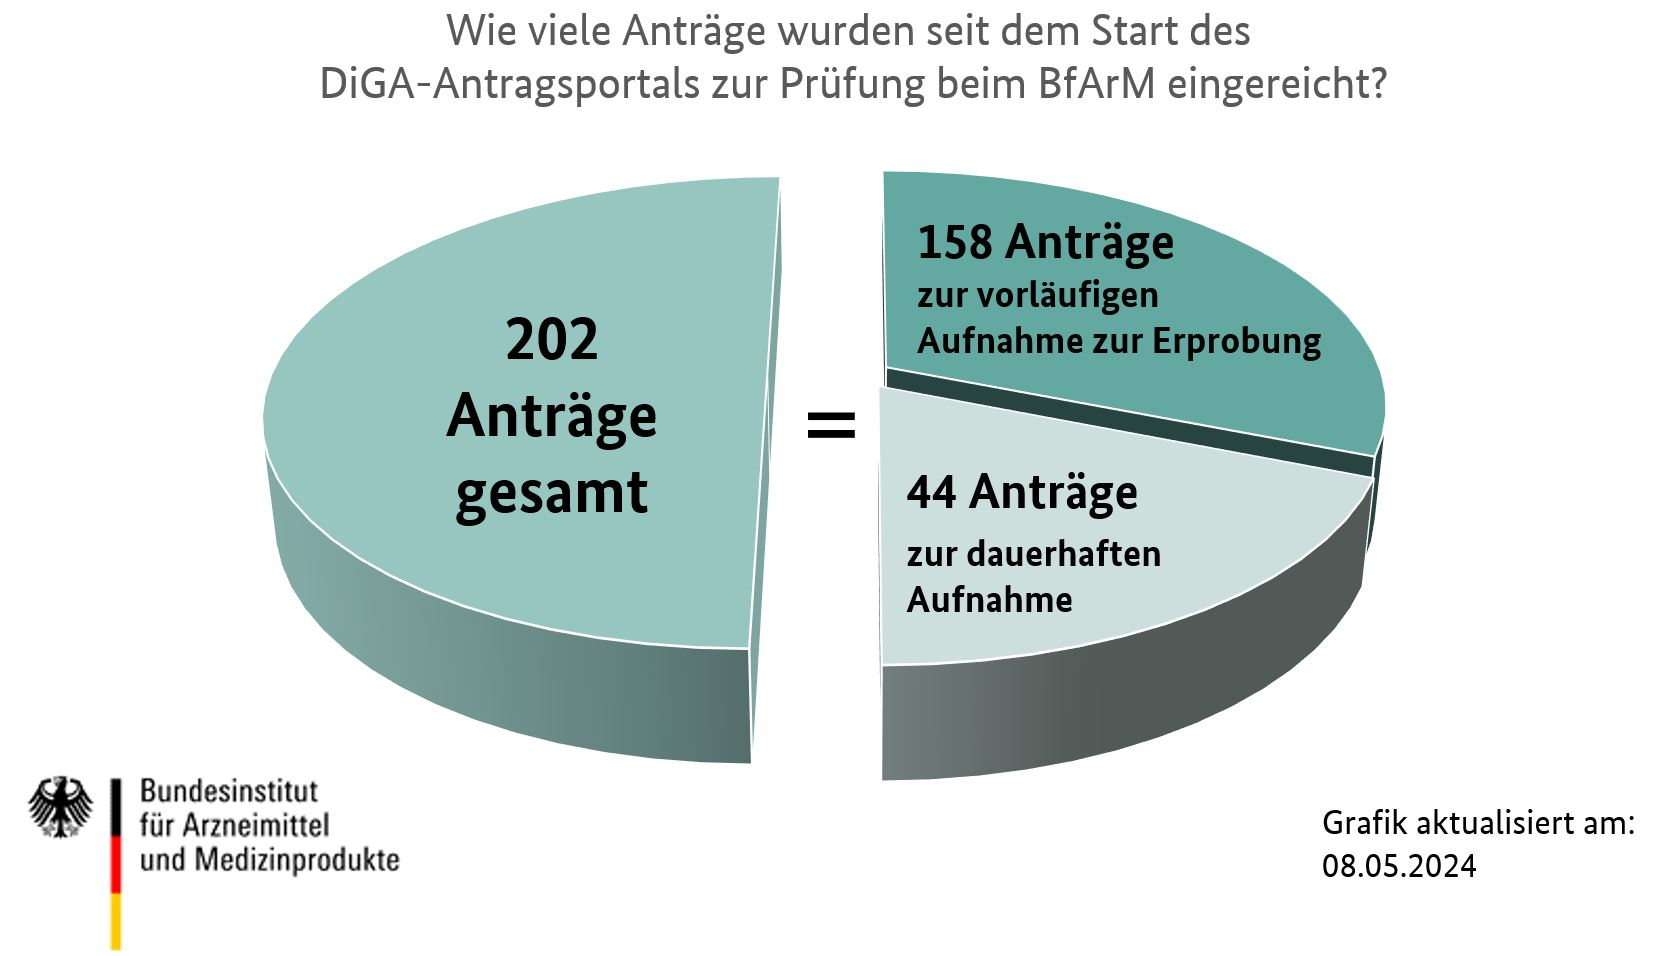
\includegraphics[width=0.75\textwidth]{./grafiken/Anzahl_Antraege_DiGA}
				\caption[Anzahl Anträge von DiGAs]{Kuchendiagramm zur Anzahl von Anträgen von DiGAs}
				\label{Abb-antragsanzahl-diga}
			\end{figure}
			In der Abbildung kann man die Aufteilung der Gesamt Anträge sehen. Von den insgesamt 202 Anträge, wurden 44 Anträge direkt dauerhaft aufgenommen. Daraus kann man schließen das circa 75 \% der Anträge, zum Zeitpunkt der Antragsanstellung, noch einen ungewissen medizinischen Nutzen hatten.
			\newpage
			\begin{figure}[htbp]
				\centering
				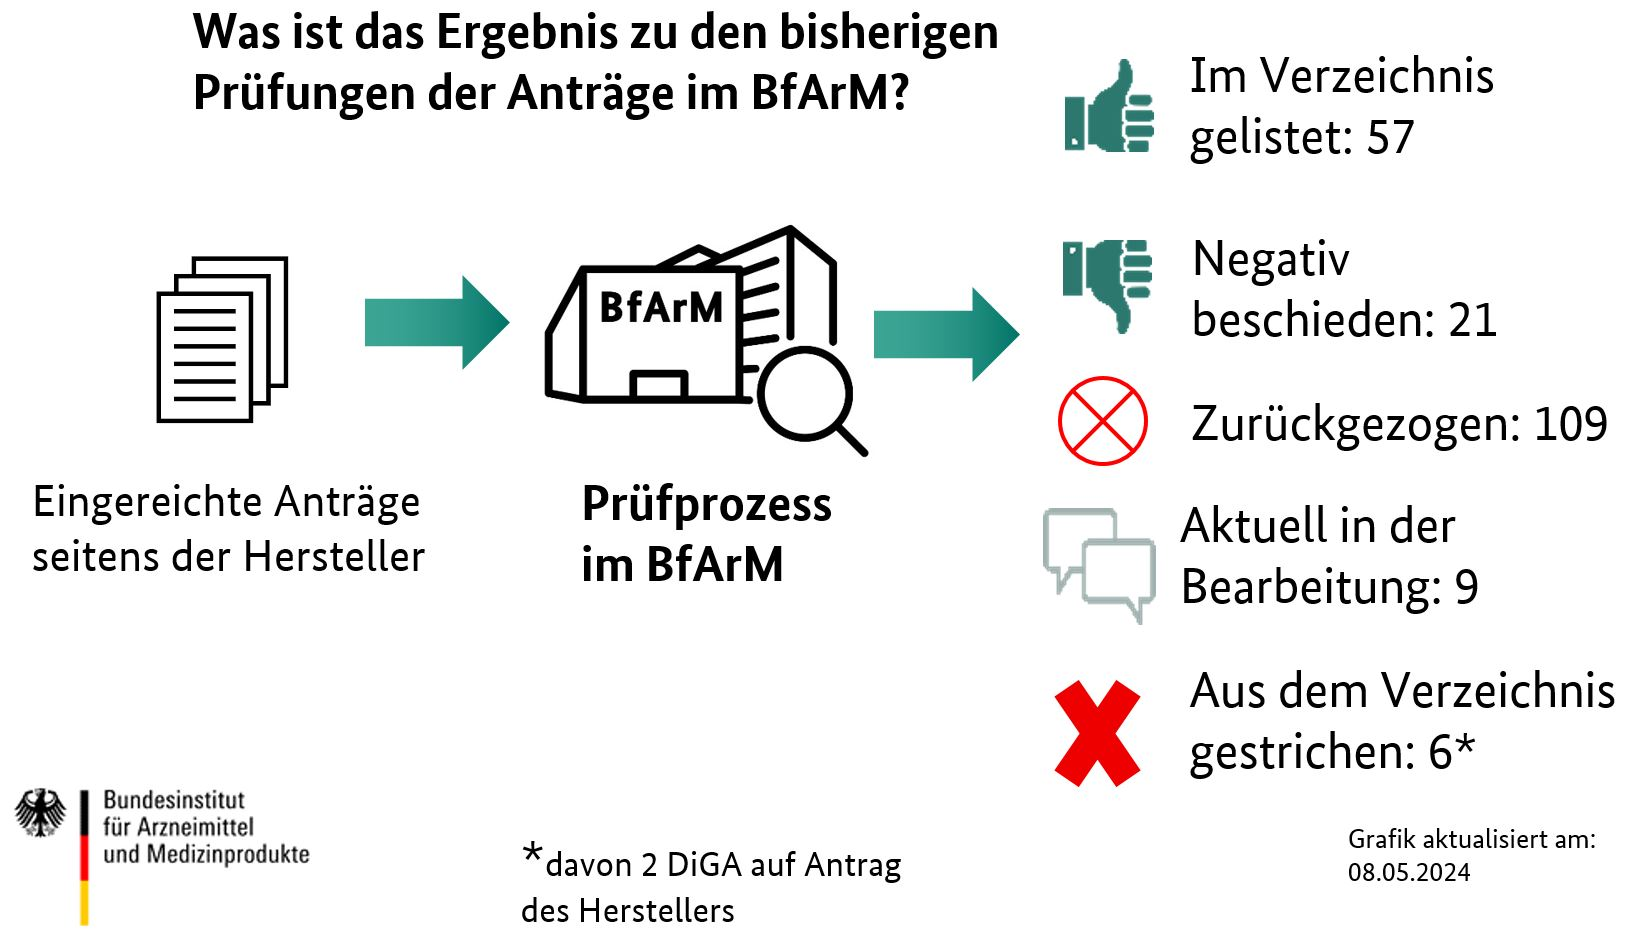
\includegraphics[width=0.75\textwidth]{./grafiken/Ergebnis_Pruefungen_DiGA}
				\caption[Abbildung zu den Ergebnissen des Fast-Track-Verfahren]{Diagramm zu den Ergebnissen des Fast-Track-Verfahren}
				\label{Abb-ergebnisse-ft}
			\end{figure} 
			In der Abbildung kann man die Prüfergebnisse, der Anträge, des BfArM sehen. Von den 202 Anträgen wurden 109 davon zurückgezogen. Somit wurden mehr als 50 \% aller Anträge von den Herstellern zurückgezogen. Laut Angaben des BfArM kommt dies durch inhaltlichen Nachbesserungsbedarf bei den Anträgen zustande, denen die Hersteller nicht rechtzeitig nachkommen konnten, aufgrund der kurzen Fristen des Fast-Track-Verfahren\cite[vgl. Z. 37]{tipps-diga-antragsansteller}   
			\newpage
			\begin{figure}[htbp]
				\centering
				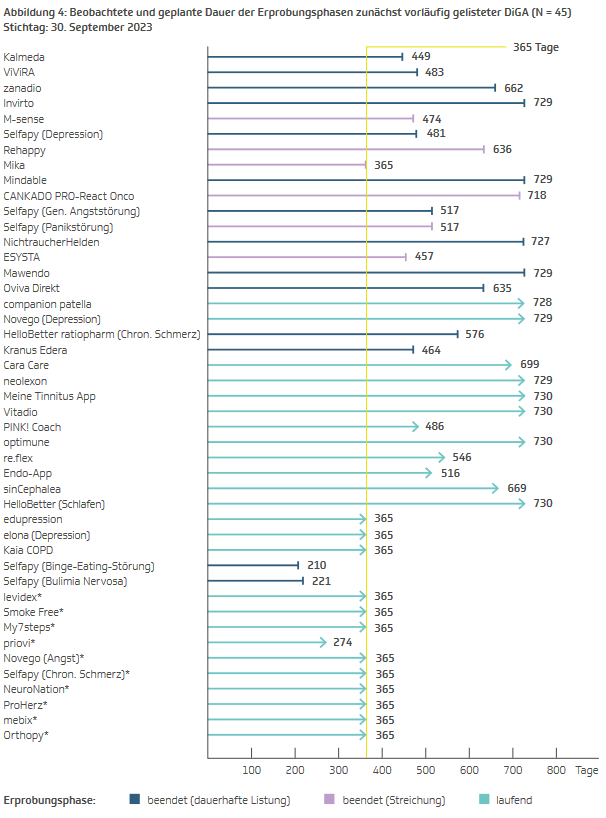
\includegraphics[height=0.75\textheight]{./grafiken/erprobungs_phase_diga}
				\centering
				\caption[Erprobungsphase von den DiGAs]{Balkendiagramm zu der Erprobungsphase der DiGAs (Stichtag: 30. September 2023)}
				\label{Abb-erprobungsphase-diga}
			\end{figure}
			In der Abbildung kann man die Beobachtete und geplante Erprobungsphase von vorläufig gelisteten DiGAs sehen. Die gelbe Linie steht im Kontext zur Abbildung, für die  Zwölfmonatige Erprobungsphase der BfArM, wie in Abbildung \ref{Abb-ft-Verfahren} zu sehen ist. Bei den DiGAs mit abgeschlossener Erprobung (30. September 2023)(blaue und pinke Linie) handelt es sich um den Zeitraum zwischen dem Listungsdatum und dem Entscheidungsdatum des BfArM, ob die DiGA dauerhaft aufgenommen oder gestrichen wird\cite[vgl. S.10]{TK-Report-2}. Von den 6 gestrichenen DiGA wurden 2 davon, auf bitte des Herstellers gestrichen wie in Abbildung \ref{Abb-ergebnisse-ft} zu sehen ist. Der Hersteller kann die Verlängerung der Erprobungsphase beantragen oder sie kann auf die Prüfphase zurückzuführen sein, die vom BfArM veranlasst wird. Um herstellerinitiierte Verlängerungen sicher zu identifizieren, wird ein Prüfzeitraum von 120 Tagen anstelle der gesetzlich vorgeschriebenen drei Monate angesetzt. Bei mehr als zwei von drei DiGA, die für die Erprobung bei Markteintritt aufgeführt sind (23 von 45), wird dieser angenommene Prüfzeitraum überschritten. Daher kann davon ausgegangen werden, dass Hersteller Verlängerungen beantragen. Es ist jedoch zu beachten, dass für zehn der 22 Anwendungen ohne bereits verlängerte Erprobungsphase zum Stichtag 30. September 2023 noch eine spätere Verlängerung möglich ist.\cite[vgl S. 10]{TK-Report-2} Wie man in der Abbildung sehen kann, ist somit die auf 1 Jahr angesetzte Erprobungsphase des BfArMs, nicht realistisch.
		\subsection{Preise und Vergütungsbeiträge der DiGAs}  
			In den ersten 12 Monaten (Erstes Listungsjahr) der DiGA, gilt ein vom Hersteller frei festgelegter Preis (sog. "tatsächlicher Preis"). Ab dem ersten Tag des 13. Monats wird der freie Herstellerpreis durch einen vom Hersteller und GKV-Spitzenverband verhandelten Vergütungsbeitrag, ersetzt. Sollte es jedoch zu keiner Einigung zwischen dem Hersteller und des GKV-Spitzenverband kommen, wird eine Schiedstelle eingeschaltet die ein Vergütungsbeitrag festlegt. Dabei ist der Vergütungsbeitrag rückwirkend, bedeutet also, sollte der Vergütungsbeitrag niedriger sein als der freie Herstellerpreis, hat die Krankenkasse einen Anspruch auf Rückzahlungen\cite[vgl. S. 11]{TK-Report-2}. Diese Preise können sich auf unterschiedliche Anwendungszeiträume beziehen, wie in Abbildung \ref{Abb-andwendungszeiträume-diga} zu sehen ist. 
			\begin{figure}[hbtp]
				\centering
				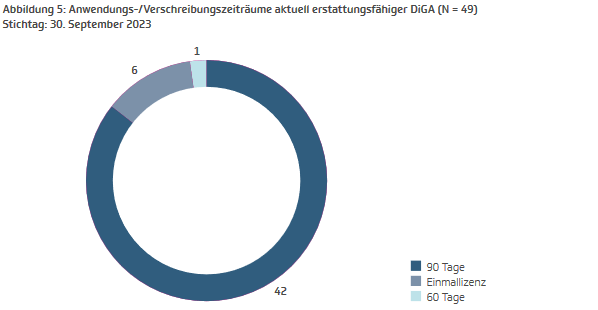
\includegraphics[width=0.75\textwidth]{./grafiken/anwendungszeitraume_diga}
				\caption[Anwendungszeiträume von DiGAs]{Kuchendiagramm zu den Anwendungszeiträume von DiGAs (Stichtag: 30. September 2023)}
				\label{Abb-andwendungszeiträume-diga}
			\end{figure}
			Sollte es nun zum Fall kommen, das die Schiedstelle eingeschaltet werden muss, um den Vergütungsbeitrag zu bestimmen, hat diese ein Preisbemessungsmodell erstellt, die die Kosten von vergleichbaren GKV-Versorgungen im jeweiligen Anwendungsgebiet untersucht. Als Beispiel war es bislang in allen Verfahren für digitale Gesundheitsanwendungen im Bereich psychischer Erkrankungen üblich, eine persönliche Gruppentherapie mit kognitiver Verhaltenstherapie als festen "Preisanker" anzunehmen. Diese Methodik wird auch in den anderen Bereichen angewendet. Die genaue Kostenberechnung für die vergleichbare Versorgung erfolgt für den Zeitraum, in dem die entsprechende DiGA genutzt wird.\cite[vgl. S. 13]{TK-Report-2} Also in der Regel 90 Tage (1 Quartal), wie in Abbildung \ref{Abb-andwendungszeiträume-diga} zu sehen ist. Basierend auf den geschätzten Kosten des Referenzpreises wird eine "Nutzenanpassung" in Form eines prozentualen Aufschlags vorgenommen. Dieser richtet sich hauptsächlich nach einer Bewertung des Ausmaßes des positiven Versorgungseffekts (gering/mittel/hoch) und der Qualität der Studien (gering/mittel/hoch), die von der Schiedsstelle vorgenommen wird. Zusätzlich zu den geschätzten Kosten des Preisankers werden auch, in Einzelfällen, andere qualitative Faktoren berücksichtigt, wie beispielsweise die Epidemiologie der Erkrankung, alternative Therapiemöglichkeiten usw. Dabei werden auch Selbstzahler- und europäische Vergleichspreise der digitalen Gesundheitsanwendungen mit einer Gewichtung von bis zu 15 \% einbezogen.\cite[vgl. S. 13]{TK-Report-2} Wie in Abbildung \ref{Tab-preise-diga} zu sehen ist, gibt es keine großen Unterschiede zwischen den Vergütungsbeiträge, die von der Schiedstelle festgelegt oder den Herstellern und GKV-Spitzenverband vereinbart wurden. 
			\begin{figure}[htbp]
				\centering
				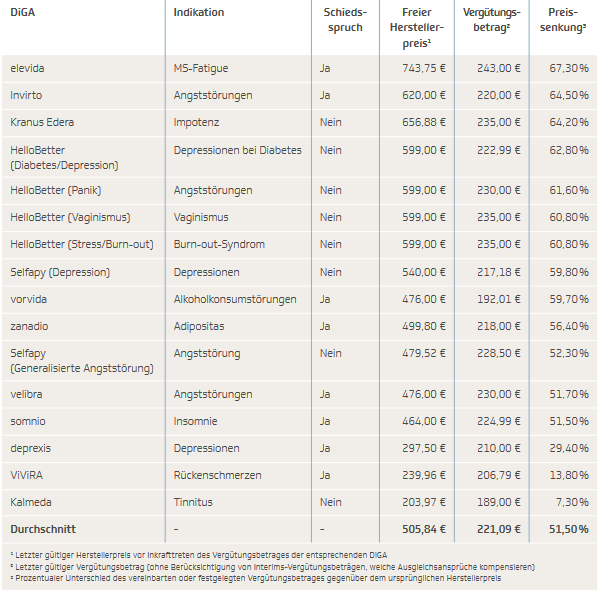
\includegraphics[width=0.75\textwidth]{./grafiken/tabelle_preise_diga}
				\caption[Gegenüberstellung der freien Herstellerpreise und verinbarten oder festgelegten Vergütungsbeiträge]{Tabelle zur Gegenüberstellung der freien Herstellerpreise und vereinbarten oder festgelegten Vergütungsbeiträge (Stichtag: 30. September 2023)}
				\label{Tab-preise-diga}
			\end{figure}
		\subsection{Anwendungsgebiete}
			\begin{figure}[htbp]
				\centering
				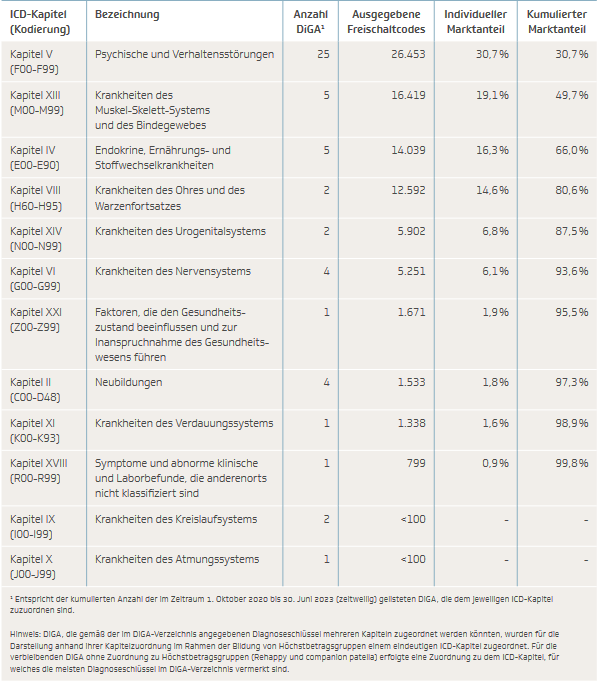
\includegraphics[height=0.75\textheight]{./grafiken/tabelle_anwendungsfelder_diga}
				\caption[Anwendungsfelder der DiGA]{Tabelle zu den Anwendungsfelder (Zeitraum: 1. Oktober 2020 - 30. Juni 2023)}
				\label{Tab-anwendungsfelder-diga}
			\end{figure}
			In der Tabelle \ref{Tab-anwendungsfelder-diga}, kann man sowohl die verteilten Freischaltcodes, als auch die Marktanteile der jeweiligen Anwendungsfelder sehen. Es wurden im angegeben Zeitraum insgesamt 86.213 Freischaltcodes ausgegeben. In der Tabelle, kann man deutlich sehen das mit circa 50 \% der DiGAs im Anwendungsfeld der Psychischen und Verhaltensstörungen sind. Diese sind mit einem Individuellem Marktanteil von 30,7 \% auch die häufigsten verordneten DiGAs.
			\newpage
			\begin{figure}[htbp]
				\centering
				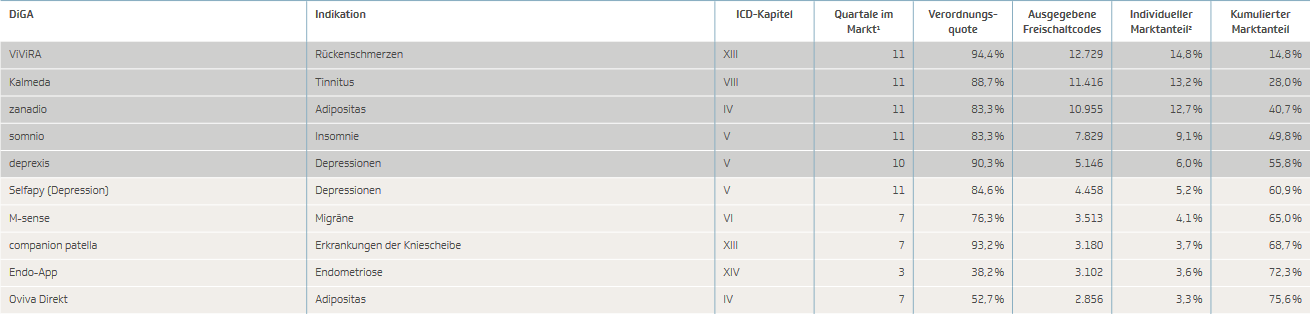
\includegraphics[width=0.75\textwidth]{./grafiken/tab_diga_verteilung}
				\caption[Freigegebene Freischaltcode je DiGA]{Tabelle zu Freigegebenen Freischaltcodes je DiGA (Zeitraum: 1. Oktober 2020 - 30. Juni 2023)}
				\label{Tab-freischaltcodes-je-diga}
			\end{figure}
			In der Tabelle kann man die Top 10 verteilten DiGAs im DiGA-Verzeichnis sehen. Diese 10 machen 75,6 \% aller ausgegeben Freischaltcodes aus. In der Tabelle wird nochmals der Marktanteil von 30,7 \% im Anwendungsfeld der Psychischen- und Verhaltensstörungen bestätigt mit somnio, deprexis und Selfapy (Depressionen).  
	\newpage
	\section{Informationen zu den Nutzern und Verordneden}
		Im folgenden Kapitel werden allgemeine Information, sowie Statistiken zu den Nutzern und Verordneden der DiGAs wiedergegeben.
		\subsection{Nutzer und Verordneden}
			\begin{figure}[htbp]
				\centering
				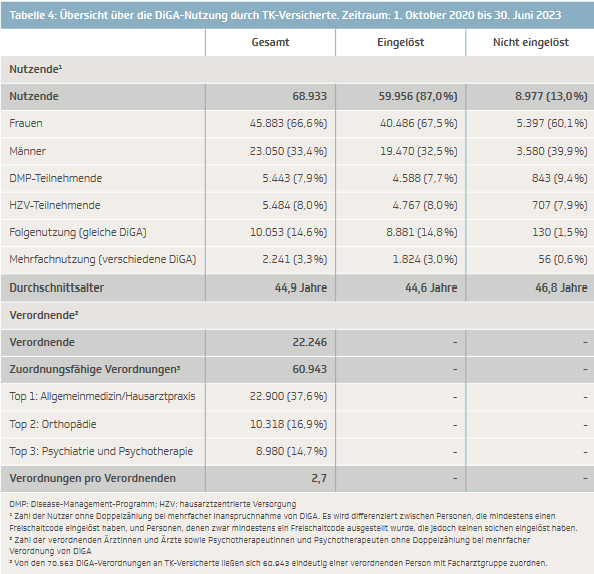
\includegraphics[width=0.75\textwidth]{./grafiken/tabelle_nutzung_versicherte_diga}
				\caption[Statistik zu den Nutzern (TK-Versicherten) und Verordneden von DiGA]{Tabelle zur Statistik zu den Nutzern (TK-Versicherten) und Verordneden von DiGA (1. Oktober 2020 - 30. Juni 2023)}
				\label{Tab-nutzung-versicherte-diga}
			\end{figure}
			In der Tabelle sieht man die Verteilung der Nutzer und aus welchen Bereichen die Verordneden kommen. Deutlich aus der Tabelle zu erkennen ist, dass $\frac{2}{3}$ der Nutzer von DiGA Frauen sind. Zusätzlich kann man noch aus der Tabelle lesen das mit fast 40 \% der größte Teil der Verordneden Hausärzte sind.
			
			Jedoch stellt man fest das dies nur 12 \% der 185.000 ertragsärztlichen Versorgung teilnehmenden Leistungserbringer. Dennoch hat sich seit den Analysen des DiGA Reports der TK 2022 (Stichtag: 30. Sptember 2021) der Anteil an teilnehmenden Verordneden, sich um den Faktor 3 erhöht. Die Verordnungsrate liegt bei 2,7 Verordnungen pro Verordnete, jedoch kann man anhand folgender Abbildung deutlich sehen, das dies nicht gleichmäßig verteilt ist
			\begin{figure}[hbtp]
				\centering
				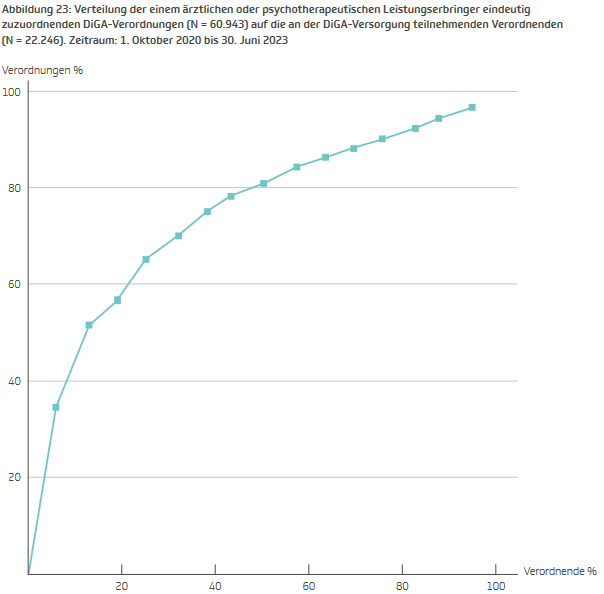
\includegraphics[width=0.75\textwidth]{./grafiken/abbildung_verordnungen_pro_verordneten_diga}
				\caption[Verordnungsverteilung (1. Oktober 2020 - 30. Juni 2023)]{Diagramm zur Verordnungsverteilung von DiGAs (1. Oktober 2020 - 30. Juni 2023)}
				\label{Abb-verordnungen-diga}
			\end{figure}
			wie man in \ref{Abb-verordnungen-diga} sehen kann. Dabei liegen 60 \% der Verordnungen bei nur circa 20 \% der Verordneden. 73,9 Prozent der verschreibenden Leistungserbringer haben innerhalb der 33 Monate des Beobachtungszeitraums maximal zwei Rezepte an TK-Versicherte ausgestellt, wobei mehr als die Hälfte (55,0 Prozent) sogar nur ein einziges Rezept ausgestellt hat. Das individuelle Verordnungsvolumen der fünf Leistungserbringer mit den meisten Verordnungen liegt zwischen 135 und 272 DiGA-Rezepten. Bundesweit gibt es nur neun Leistungserbringer, die mindestens 100 Rezepte an TK-Versicherte ausgestellt haben. Es ist festzustellen, dass die Leistungserbringer, die DiGA häufiger in ihrer Patientenversorgung einsetzen, in der Regel mehrere unterschiedliche DiGA verschreiben. Drei der fünf Leistungserbringer mit den meisten Verordnungen haben verschiedene DiGA verschrieben. Unter allen Leistungserbringern, die mindestens zwei DiGA-Rezepte ausgestellt haben (45,0 Prozent aller Verordnenden), haben 55,0 Prozent mehrere unterschiedliche DiGA verschrieben. \cite[vgl. S. 28]{TK-Report-2}
			\newpage
		\subsection{Vergleich von Nutzern und Nicht-Nutzern von DiGA}
			\begin{figure}[htbp]
				\centering
				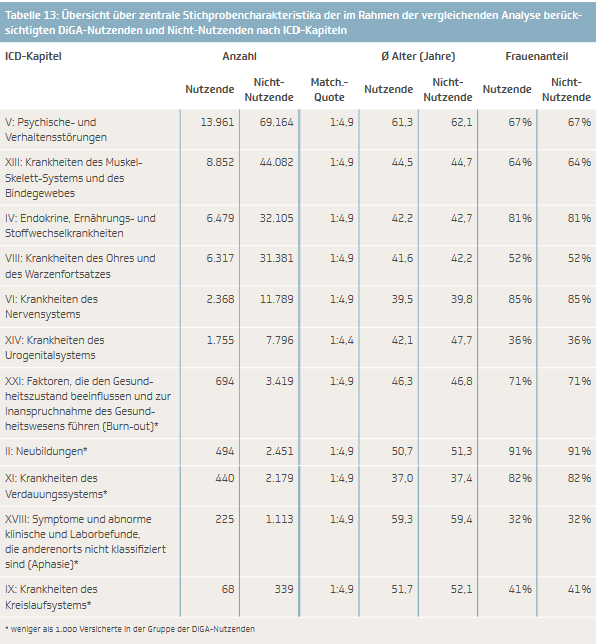
\includegraphics[width=0.75\textwidth]{./grafiken/tabelle_vergleich_nutzer_nicht_nutzer_diga}
				\caption[Stichprobencharakteristik von Nutzer und Nicht-Nutzer]{Tabelle zur Stichprobencharakteristik von Nutzer und Nicht-Nutzer}
				\label{Tab-stichprobe-diga}
			\end{figure}
			Für die Mehrheit der verschiedenen Anwendungsgebiete zeigen sich bei der Morbidität ähnliche Muster zwischen Nutzern und Nicht-Nutzern. Dabei weist die Gruppe der DiGA-Nutzer in sechs von elf Anwendungsbereichen während des Beobachtungszeitraums – bei einer durch Matching nahezu gleichen Altersverteilung (siehe Abbildung \ref{Tab-stichprobe-diga}) – einen signifikant niedrigeren Komorbiditätsgrad auf, gemessen mit dem Charlson-Komorbiditätsindex (Charlson Comorbidity Index, CCI). Wenn man nur die sechs Anwendungsbereiche betrachtet, in denen mindestens 1.000 Versicherte in der Gruppe der DiGA-Nutzer sind, trifft dies auf zwei Drittel der ICD-Kapitel zu. In den Bereichen der endokrinen, Ernährungs- und Stoffwechselkrankheiten sowie der Krankheiten des Ohres und des Warzenfortsatzes gibt es nur minimale Unterschiede zwischen DiGA-Nutzern und Nicht-Nutzern. Obwohl es statistisch signifikante Unterschiede gibt, sind die absoluten Unterschiede im Charlson-Komorbiditätsindex (CCI) in den meisten Anwendungsbereichen extrem gering. Bei sechs der elf ICD-Kapitel sind diese Unterschiede so gering, dass sie nur die zweite Nachkommastelle betreffen. Insgesamt gibt es dadurch keine klinisch relevanten Unterschiede in den Morbiditätsprofilen der Vergleichsgruppen.\cite[vgl. S. 36]{TK-Report-2}
			\newpage
		\subsection{Leistungsinanspruchnahmen von Nutzer und Nicht-Nutzern}
			Trotz eines ähnlichen Morbiditätsprofils haben DiGA-Nutzer im Kalenderjahr vor der ersten DiGA-Nutzung in den meisten der analysierten Indikationsgebieten, in einzelnen Versorgungsbereichen, eine deutlich höhere Leistungsinanspruchnahme als die Kontrollgruppe der Nicht-Nutzer. Gerade in der Ambulanten Vertragsärztlichen Versorgung ist dies deutlich festzustellen. Zusätzlich zeigen DiGA-Nutzer eine höhere Tendenz zu Arbeitsunfähigkeitstagen, als Nicht-Nutzer.\par
			Bei 5 von den 6 Indikationsgebieten mit Minimum 1.000 Versicherten in der Gruppe der DiGA-Nutzer, liegt die durchschnittliche Anzahl der dokumentierten Arztkontakte deutlich höher als bei der Vergleichsgruppe der Nicht-Nutzer. Je nach Indikationsgebieten hatten dabei die DiGA-Nutzer im Schnitt 1,6 (Psychische- und Verhaltensstörungen) bis 6,1 (Krankheiten des Nervensystems) mehr Kontakte zu vertragsärztlichen Leistungserbringern, pro Kalenderjahr, als die Nicht-Nutzer der Vergleichsgruppe. Jedoch ist einem Indikationsgebiet mit mehr als 1.000 DiGA-Nutzern (Krankheiten des Urogenitalsystems) kein deutlicher Unterschied zwischen Gruppen der DiGA-Nutzer und Nicht-Nutzer zu verzeichnen. Zusätzlich gibt es eine deutlich niedrigere Zahl der ambulanten Arztkontakte des Indikationsgebiets XXI, bei dem es nur die Anwendungen Better Stress und Burn-out (Burn-out-Syndrom) gibt. Darüber hinaus ist es  auffällig dass in 10 der 11 betrachteten Indikationsgebieten die absolute Differenz von DiGA-Nutzern und Nicht-Nutzern bei den Facharztkontakten größer ausfällt, als bei den Hausarztkontakten.\par 
			Deutliche Unterschiede zeigen sich auch in der Inanspruchnahme von Arbeitsunfähigkeitstagen in 4 von 6 der Indikationsgebieten mit mindestens 1.000 DiGA-Nutzern. Hierbei kommen die DiGA-Nutzer in den jeweiligen Indikationsgebieten im Beobachtungszeitraum auf 4,8 (Psychische- und Verhaltensstörungen) bis 7,6 (Krankheiten des Nervensystems) Arbeitsunfähigkeitstage mehr im Jahr, als die Gruppe der Nicht-Nutzer. Anzumerken ist, das im Indikationsgebiet der Neubildungen (ICD-10 C00-C97) eine mit 21,8 Tagen signifikant höhere Anzahl der Arbeitsunfähigkeitstage zu verzeichnen ist als bei den Nicht-Nutzern. Hierbei ist jedoch in Betracht zu ziehen, das im Vergleich nur 494 DiGA-Nutzer berücksichtigt werden konnten.\par
			Betrachtet man die durchschnittliche Anzahl der Krankenhaustage und auf die verabreichten Arzneimittel-Tagesdosen (Defined Daily Dose, DDD) im Kalenderjahr, fällt die Tendenz zur erhöhten Inanspruchnahme durch DiGA-Nutzer weniger auf. Die durchschnittliche Differenz zwischen DiGA-Nutzern und Nicht-Nutzern beläuft sich hierbei nur auf 0,8 Tage. Ein Ausreißer hierbei ist, wie bei den ambulanten Arztkontakten, das Indikationsgebiet XXI, wo wieder ein signifikant niedrigerer Wert für Krankenhaustage zu verzeichnen ist zwischen DiGA-Nutzern und Nicht-Nutzern.\par
			Bei der Inanspruchnahme von Arzneimittel liegen bei 4 Indikationsgebiete deutliche Unterschiede vor. Bei Krankheiten des Ohres und des Warzenfortsatzes (-27 DDD), sowie Krankheiten des Urogenitalsystems (-204 DDD) ist ein signifikant niedrigerer Wert für DDD zu dokumentieren, als bei der Vergleichsgruppe von Nicht-Nutzern. Bei endokrinen, Ernährungs- und Stoffwechselkrankheiten, sowie Krankheiten des Nervensystems (+90 DDD) ist eine signifikant erhöhte DDD zu verzeichnen, als bei der Vergleichsgruppe von Nicht-Nutzern.\par
			Insgesamt zeigen die vergleichenden Analysen Unterschiede in den Versorgungsstrukturen von DiGA-Nutzern und Nicht-Nutzern auf. In diesen sieht man die erhöhte Tendenz von DiGA-Nutzer zur Inanspruchnahme pro Kalenderjahr im Vergleich zu Nicht-Nutzern, trotz eines gleichen oder ähnlichen Morbiditätsprofil. Um die speziellen Versorgungsbedürfnisse von DiGA-Nutzerinnen und -Nutzern, ihre Ursachen und insbesondere die Veränderungen nach der Nutzung einer DiGA genauer zu untersuchen, ist zusätzliche qualitative und quantitative Versorgungsforschung erforderlich. Dabei sollen auch Aspekte berücksichtigt werden, die zum aktuellen Zeitpunkt noch nicht analysiert werden konnten.
			\newpage
	\section{Der Status Quo von DiGA in anderen Ländern}
		Die Einführung der "App auf Rezept" als Regelleistung der Gesetzlichen Krankenkasse ist nicht nur in Deutschland eine Neuheit. Auch International betrachtet, sind die konzeptionierten Regelungen für die Vergütung von Anwendungen, sowohl App als auch Web, zur Unterstützung der Behandlung und Managements von Krankheiten in der Form einzigartig. Seit der Einführung des Digitalen-Versorgungs-Gesetz und somit auch von DiGAs, wurde die Entwicklung dessen mit großem Interessen auch von anderen Ländern verfolgt und hierbei insbesondere von den Europäischen Nachbarländern. Zu den Ländern die sich bereits intensiv mit der Implementierung von DiGAs beschäftigt haben zählen Frankreich, Belgien, Liechtenstein und Schweden.\cite[vgl. S.25-26]{TK-diga-report-1}
		\subsection{PECAN-Verfahren}
			\begin{figure}[htbp]
				\centering
				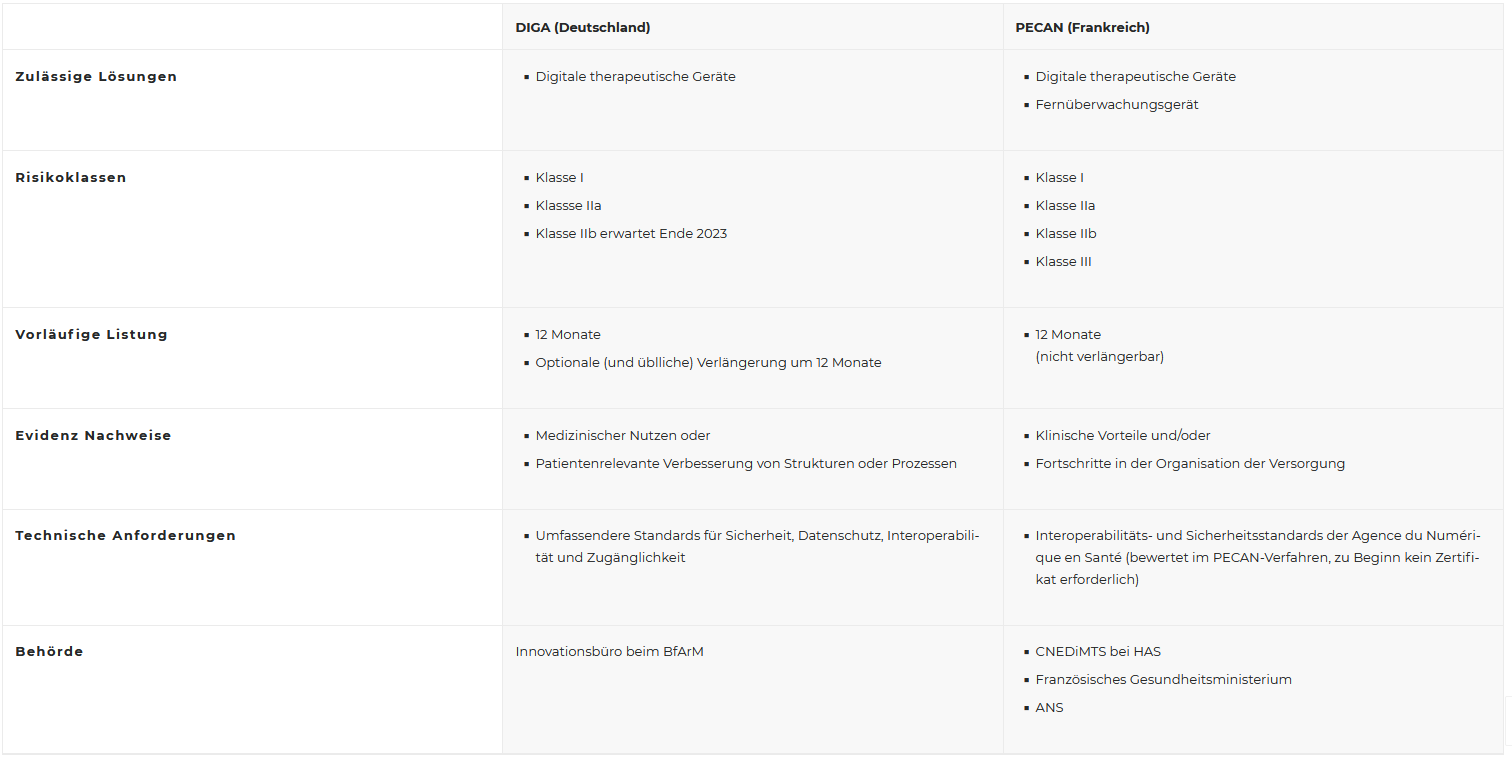
\includegraphics[width=0.75\textwidth]{./grafiken/abbildung-diga-versus-pecan}
				\caption[DiGA vs. PECAN]{Abbildung zum Vergleich von DiGA und PECAN}
				\label{Abb-diga-vs-pecan}
			\end{figure}
			Das Französische PECAN-Verfahren (Prise en Charge Anticipée Numerique des Dispositifs Médicau, Digitale Frühförderung für Medizinprodukte) ist das äquivalent zum Deutschen DiGA-Verfahren. Hierbei ist anzumerken, das weitreichende Unterschiede im PECAN-Verfahren gibt. Der Erste große Unterschied zwischen beiden Verfahren ist, dass das PECAN-Verfahren auch zusätzlich für Telemedizinprodukte verwendet werden kann, wie man in Abbildung \ref{Abb-diga-vs-pecan} zu sehen ist. Zusätzlich erlaubt das PECAN-Verfahren die Einbeziehung von Anwendungen die für die Risikoklassen 2b und 3 bestimmt sind. Eine Abweichung gibt es zusätzlich in der Regelung der vorläufigen Listung. Wo im DiGA-Verfahren eine zusätzliche Verlängerung von 12 Monaten, zu den ursprünglichen 12, möglich ist, ist dies beim PECAN-Verfahren nicht möglich. Weiterhin fordert das PECAN-Verfahren, zusätzlich zum CE-Kennzeichen, das die Anforderungen für Interoperabilitäts- und Sicherheitsstandards der Agence du Numérique en Santé erfüllt sind. Der wahrscheinlichst größte bis jetzige Unterschied zwischen dem DiGA- und PECAN-Verfahren ist, das die Anwendung in Frankreich noch nicht erstattet wird.\cite{PECAN-Verfahren}
		\subsection{DtX in den USA}
			DTx (Digital Therapeutics) sind Mobile Health Anwendungen die durch die FDA freigegeben wurden. Hierbei ist jedoch anzumerken, dass bis zum jetzigen Zeitpunkt es kein CFR-spezifische (CFR: Code of Federal Regulations) Regulierungsmethode zur freigabe von DTx gibt. DTx werden bis zum jetzigen Zeitpunkt wie Medizinische Geräte der Kategorie 2 (Stellen ein moderates Risiko für Gesundheit dar) unter "CFR Title 21 Subchapter H" reguliert, was bedeutet, dass diese eine verpflichtende "FDA pre-marketing submission" durchlaufen müssen. Diese beinhalten eine 6 - 12 Monatige Überprüfungszeit (Basierend auf den vorhergesehenen Zielmarkt) und Kosten zwischen 3.000 für kleinere und 113.000 US-Dollar für große Unternehmen.\par
			Ende 2020 wurde das "Digital Health Center of Excellence" (DHCoE) von der FDA etabliert. Die DHCoE unterstützt vor allem die Einhaltung von FDA Regularien und hilft auch den Entwicklern digitale Gesundheitsinnovationen zu Nutzerfreundlichen tools umzuwandeln. Durch die Arbeit des DHCoE wurde unter anderem die PDTx (Prescribed Digital Therapeutics) möglich. Die PDTx kommt zu einem äquivalent einer DiGA am nächsten, denn diese erfüllen alle Anforderungen an einer DTx, aber werden auch von Ärzten anerkannt und verschrieben. Die erste PDTx kam Ende 2017 raus und bis zum jetzigen Zeitpunkt gibt es circa 40 PDTx die von der FDA freigegeben wurden.\par
			Ein großes Problem derzeitig für die Nutzung von sowohl DTx als auch PDTx ist das U.S. Gesundheitssystem. Dadurch das nicht eine einheitliche, nationale Krankenkasse gibt, müssen die Hersteller zusätzlich zur FDA Freigabe noch ihr Produkt im freien Markt unter Beweis stellen.\cite{dtx-usa}
	\section{Fragen}
		\subsection{Wie hoch ist die Verschreibungshäufigkeit?}
			\begin{figure}[htbp]
				\centering
				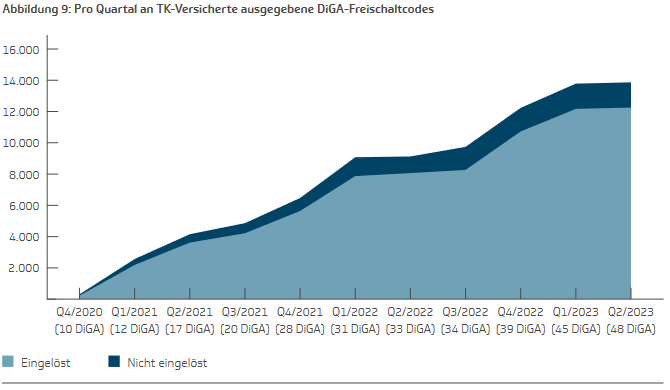
\includegraphics[width=0.75\textwidth]{./grafiken/abbildung-verschreibungstrend}
				\caption[Ausgegebene Freischaltcodes im Quartal]{Diagramm zu ausgegebenen Freischaltcodes im Quartal}
				\label{Abb-verschreibungstrend}
			\end{figure}
			Seit der 1. DiGA Verschreibung 2020, gibt es einen eindeutigen Aufwärtstrend, wie in Abbildung \ref{Abb-verschreibungstrend} zu sehen ist. Die Verordnungen sind im durchschnitt um 20 \% pro Quartal gestiegen. Jedoch kommen circa 60 \% aller Verschreibungen auf nur 20 \% der Verordnungsfähigen Ärzten, wie in Kapitel 3.1 beschrieben. Zusätzlich anzumerken ist, das mit circa 40 \%, die Hausärzte den größten Teil bei den Verschreibungen ausmachen. Im Allgemeinen kommt es auf einen Schnitt von 2,7 Verordnungen pro Arzt im Zeitraum des 1. Oktobers 2020 bis zum 30. Juli 2023   
		\subsection{Wer nutzt DiGAs und welche kommen dabei zu Einsatz?}
			Die meisten Verschreibungen sind im Bereich der Psychischen- und Verhaltensstörungen, gefolgt von Krankheiten des Muskel-Skelett-Systems und des Bindegewebes, wie in Tabelle \ref{Tab-anwendungsfelder-diga} in Kapitel 2.3 zu sehen ist. Die größte Gruppe der Nutzende liegt mit 66 \% bei Frauen mit einem Durchschnittsalter von circa 45 Jahren, wie in Kapitel 2.3 beschrieben. Schaut man sich dazu noch die Top 10 der meist verschriebenen DiGA (Tabelle \ref{Tab-freischaltcodes-je-diga}), sieht man deutlich das die DiGA für die Begleiterscheinungen des Alterns konzipiert wurden und erklärt die hohe Verschreibungsrate.                       
		\subsection{Helfen DiGA?}
			Nimmt man alle Informationen die in Kapitel 3 und dessen unter Kapitel beschrieben sind zusammen, könnte man die Frage mit einem Ja beantworten. Aber um eine eindeutige Antwort auf die Frage zu bekommen, müsste man dennoch eine Feldstudie zur Wirksamkeit von DiGA machen. Zwar müssen alle DiGA, seien sie nur vorzeitig oder dauerhaft gelistet, einen medizinischen Nutzen nachweisen, dennoch konnte nicht nachgewiesen werden das der bessere Charlson-Komorbiditätsindex Wert von DiGA-Nutzern auch tatsächlich den DiGAs zu verschulden ist. Dies könnte auch an der erhöhten Inanspruchnahme von Leistungen wie Krankenhaus Tagen, Ambulanten Arztbesuche oder ähnlichem liegen.        
		\subsection{Wie steht Deutschland im Vergleich zu anderen Ländern?}
			Deutschland ist im Vergleich zu anderen Ländern ein Vorreiter im Bereich der Digitalen Gesundheitsanwendungen. Zwar gibt es die erste "offizielle" DiGA schon seit 2017 die die FDA freigegeben hat in den USA, jedoch war Deutschland das erste Land, dass ein maßgeschneidertes Verfahren für Digitale Gesundheitsanwendungen entwickelt hat. International wird diese Entwicklung mit großem Interesse verfolgt. Länder wie Schweden, Belgien, Liechtenstein und neulich auch Österreich haben bereits ein äquivalentes Verfahren entwickelt. Ein gutes Beispiel wäre Frankreich mit dem PECAN-Verfahgren, das auch für die Zulassung für Telemedizinprodukte verwendet wird und auch für mehr Risikoklassen konzipiert wurde. Ein Manko hierbei wäre jedoch das die Produkte von der Krankenkasse nicht vergütet werden. Besonders Überraschend an Deutschlands Vorreiter rolle war, das die USA noch keinerlei ähnliches Verfahren für Digitale Gesundheitsanwendungen. Dies ist aber mit hoher Wahrscheinlichkeit dem einzigartigen Gesundheitssystem der USA zu verschulden.     
	\section{Fazit}
		Im Allgemeinen sind DiGA eine zukunftsweisende Technologie für das Gesundheitssystem. Es besteht aber weiterhin Verbesserungsbedarf beim der Implementation des Fast-Track-Verfahren gerade in Hinsicht der Hersteller. Den bis jetzt wurden fast 50 \% aller gestellten Anträge vom Hersteller selbst zurückgezogen, da die Fristen zur Überarbeitung der Anträge im Fast-Track-Verfahren einfach zu kurz waren. Ein weiteres großes Problem derzeit ist, die Unwissenheit / Missinformationen, die die Ärzte und auch Nutzer über DiGAs haben. In meiner Recherche zu DiGAs hat sich nämlich herauskristallisiert, das die Ärzte die bis jetzt noch keinerlei DiGA verschrieben haben, nicht mal wussten das es diese gibt oder sich bewusst dagegen entschieden haben, da sie die Medizinische Wirksamkeit von DiGA in Frage gestellt haben. Auch auf Seiten der Nutzer gibt es noch Schwierigkeiten, denn diese wissen teilweise auch nicht das es DiGA gibt. Dagegen lässt sich aber mit Workshops / Infotage für Ärzte Abhilfe schaffen. Daraufhin können dann auch die Ärzte die Nutzer über die DiGAs aufklären. Was jedoch noch, meiner Meinung nach, gemacht werden muss, sind qualitative Feldstudien zur medizinischen Wirksamkeit von DiGAs wie in der Frage: "Helfen DiGA?" beschrieben. Sollten diese Probleme behoben werden hat die Technologie DiGA absolut das Potenzial ein Pfeiler der modernen Gesundheitsversorgung zu werden, indem diese die Ärzte entweder bei der Behandlung von Krankheiten unterstützt oder diese sogar entlastet.        
		          
			   	 
\bibliographystyle{abbrv}
\bibliography{seminar_arbeit_marcelo}
\end{document}